\documentclass{beamer}
\usetheme{Montpellier}

\usepackage{color}
\usepackage{amsfonts}
\usepackage{comment}

%%% Al parecer necesito esto en ubuntu para los acentos
%\usepackage[spanish]{babel}
%\selectlanguage{spanish}
%\usepackage[utf8]{inputenc}

\definecolor{myblue}{rgb}{0.25, 0, 0.75}
\definecolor{mygold}{rgb}{1,0.8,0.2}
\definecolor{gray}{rgb}{0.5, 0.5, 0.5}
\definecolor{lucia}{rgb}{0.8,0.4,0.7} 

\newcommand{\myurl}[1]{\href{http://#1}{\textcolor{gray}{\texttt{#1}}}}
\newcommand{\myem}[1]{\structure{#1}}
\newcommand{\myurlshort}[2]{\href{http://#1}{\textcolor{gray}{\textsf{#2}}}}

\newcommand{\RPackage}[1]{\textcolor{gray}{\textsf{#1}}}
\newcommand{\pl}[1]{\texttt{#1}}
\newcommand{\RCode}[1]{\texttt{#1}}
\newcommand{\RFunction}[1]{\textsf{#1}}
\newcommand{\RClass}[1]{\textcolor{mygold}{\textsf{#1}}}
\newcommand{\BIOCfunction}[1]{\textcolor{orange}{#1}}

\setbeamercolor{example text}{fg=lucia}
\setbeamertemplate{sections/subsections in toc}[ball unumbered]
\setbeamertemplate{frametitle continuation}[from second][]
\setbeamertemplate{itemize subitem}[triangle]
\setbeamertemplate{footline}[page number]
\setbeamertemplate{caption}[numbered]
\setbeamertemplate{navigation symbols}{}

\renewcommand{\footnotesize}{\fontsize{6.10}{12}\selectfont}

\def\argmax{\operatornamewithlimits{arg\,max}}
\def\argmin{\operatornamewithlimits{arg\,min}}

%%\bibliographystyle{plain}


\title{Seminar III: R/Bioconductor}
\author{Leonardo Collado Torres \\ lcollado@lcg.unam.mx \\  Bachelor in Genomic Sciences \\ \myurl{www.lcg.unam.mx/\string~lcollado/}}
\date{
August - December, 2009
}








\usepackage{Sweave}
\begin{document}

\begin{frame}[allowframebreaks]
  \titlepage
\end{frame}

\section*{Class outline}

\begin{frame}[allowframebreaks]
  \frametitle{Bioconductor and Documentation}
  \tableofcontents[hideallsubsections]
\end{frame}

%%%%%%%%%%%%%%%%%%%%%%%%%%%%%%%%%%%%%%%%%%%%%%%%%%%%%%%%%%%%%%%%%%%%%%%%%%%
\section{Bioconductor}

\begin{frame}[allowframebreaks]
  \frametitle{Intro}
  \begin{itemize}
  \item It's the largest repository of \alert{genomic} related packages for \pl{R} available at \url{http://bioconductor.org}.
  \item BioC was founded in 2001 and here you can find the core \myurlshort{bioconductor.org/overview/coredevs}{developers}. Just like \pl{R}, it follows a 6 month release cycle.
  \item I highly \emph{recommend} you to visit the basic introduction \myurlshort{bioconductor.org/docs/faq/}{here}\footnote{Scroll down to the \emph{What is Bioconductor?} section}.
  \item It's open source and open development initiative! \emph{You} can contribute to BioC!
  \end{itemize}
\end{frame}

\begin{frame}[allowframebreaks, fragile]
  \frametitle{Getting started}
  \begin{itemize}
  \item In \pl{R}, the basic function to install a packages is without much surprise \BIOCfunction{install.packages()}
  \item For Bioconductor, use the \alert{biocLite} script. You might find this \myurlshort{bioconductor.org/docs/install/}{guide} useful :)
\begin{Schunk}
\begin{Sinput}
> source("http://bioconductor.org/biocLite.R")
> biocLite()
\end{Sinput}
\end{Schunk}
  \item Using \pl{biocLite} without any arguments downloads a basic set of packages for your appropiate \pl{R} version and plataform.
  \end{itemize}
\end{frame}  

\begin{frame}[allowframebreaks]
  \frametitle{Browising for packages}
  \begin{itemize}
  \item If you are looking for a package that might help you with your work, I recommend these two options:
  \begin{enumerate}
  \item While very new, the \pl{biocViews} taxonomy browser is very promising and easy to browse: \myurlshort{bioconductor.org/packages/2.5/Software.html}{software 2.5 biocViews} and \myurlshort{wiki.fhcrc.org/bioc/biocViews_categories}{biocViews categories}
  \item Currently, the most complete option is to simply browse the \myurlshort{bioconductor.org/download}{download} section. For example, software for the current dev version (BioC 2.5).
  \end{enumerate}
  \item A package can \emph{depend}, \emph{import} and \emph{suggest} other packages.
  \begin{enumerate}
  \item Depend: end user can see the functions
  \item Import: the package uses but does not let the end user see
  \item Suggest: useful for some expanded workflows
  \end{enumerate}
  \item On which packages does \BIOCfunction{chipseq} depend on?
  \item What is the 5th most downloaded Bioconductor package?
  \end{itemize}
\end{frame}

\begin{frame}[allowframebreaks, fragile]
  \frametitle{Viewing a package}
  \begin{itemize}
  \item As for any package you've installed, you can view a basic description, the list of functions and methods with the following syntax:
\begin{Schunk}
\begin{Sinput}
> help(package = pkgname)
\end{Sinput}
\end{Schunk}
  \item Who is the maintainer of the \pl{Biostrings} package? 
  \item Her or his email?
  \item How is it licensed?
  \end{itemize}
\end{frame}

\begin{frame}[allowframebreaks]
  \frametitle{Package documentation}
  \begin{itemize}
  \item A \alert{BIG} difference between Bioconductor packages and regular CRAN packages is that Bioconductor packages are documented with a \emph{vignette} file and a reference manual.
  \item A \BIOCfunction{vignette} is a document that contains both text (explanations) and \pl{R} code that exemplify how to use the functions from a given package.
  \item The \BIOCfunction{reference manual} lists all the functions/methods with some examples but can be harder to understand.
  \end{itemize}
\end{frame}

\begin{frame}[allowframebreaks, fragile]
  \frametitle{Finding vignettes}
  \begin{itemize}
  \item While the pdf files are normally built on your machine, you can also download them by browsing the \myurlshort{bioconductor.org/download}{download} section.
  \begin{itemize}
  \item For example look \myurlshort{bioconductor.org/packages/devel/bioc/html/chipseq.html}{here} for the chipseq vignette\footnote{More exactly, a workflow.}.
  \end{itemize}
  \item Inside \pl{R}, you can also find the list of available vignettes by typing:
\begin{Schunk}
\begin{Sinput}
> vignette(package = "pkgname")
\end{Sinput}
\end{Schunk}
  \item \alert{Note:} if you are using the dev version (such as us), checking the \pl{Bioconductor Changelog} for a package can be informative!
  \item What kind of bug did they fix on August 4th?
  \end{itemize}
\end{frame}

\begin{frame}[allowframebreaks]
  \frametitle{Expert help}
  \begin{itemize}
  \item If you have explored every way to find help, there is a way to get expert help!
  \item Have you really, really, yes \ldots really explored \alert{all} the options? Obviously including a google search. Reading the \myurlshort{bioconductor.org/docs/postingGuide.html}{posting guide} is a must!
  \item Then, simply send your question to the \myurlshort{bioconductor.org/docs/mailList.html}{Bioconductor Mailing List}. There are three flavors:
  \begin{enumerate}
  \item General bioconductor list
  \item BioC-devel list
  \item High throughput sequencing list
  \end{enumerate}
  \end{itemize}
\end{frame}

\begin{frame}[allowframebreaks]
  \frametitle{Registering to the list}
  \begin{itemize}
  \item At least during this semester, I will require \alert{all of you} to register to the \myurlshort{bioconductor.org/docs/mailList.html}{BioC mailing list}.
  \item As you could see on the syllabus, from next class on forth, I will ask some of you to present interesting topics from the discussions of that week.
  \item So, go to this URL: \url{https://stat.ethz.ch/mailman/listinfo/bioconductor} 
  \item Enter your information and I \alert{highly} recommend you to choose "Yes" for the option: \pl{Would you like to receive list mail batched in a daily digest?} 
  \end{itemize}
\end{frame}

\begin{frame}[allowframebreaks]
  \frametitle{Extra}
  \begin{itemize}
  \item Feel free to register to the other two mailing lists: 
  \item \url{https://stat.ethz.ch/mailman/listinfo/bioc-devel}
  \item \url{https://stat.ethz.ch/mailman/listinfo/bioc-sig-sequencing}
  \item You may decide to \emph{filter} the emails into a specific folder in your mail :) 
  \end{itemize}
\end{frame}

\begin{frame}[allowframebreaks]
  \frametitle{Workshops}
  \begin{itemize}
  \item In accordance with the open source nature of Bioconductor, you can find presentations, talks, labs and much more on the \BIOCfunction{Workshops} page.
  \item \url{http://bioconductor.org/workshops/}
  \item If you browse to 2008 and 2009, you'll notice some familiar courses :)
  \item For the curious ones, the BioC workshops such as BioC2008 and BioC2009 have very interesting labs. A lab is a practical session.
  \end{itemize}
\end{frame}

\begin{frame}[allowframebreaks]
  \frametitle{Workflows}
  \begin{itemize}
  \item Although partially contained on the workshops section, Bioconductor has a set of freely available workflows.
  \item \url{http://bioconductor.org/docs/workflows/}
  \item For example, there are workflows for \pl{Affymetrix SNP arrays}, \pl{Illumina Expression Microarrays}, etc.
  \end{itemize}
\end{frame}

\begin{frame}[allowframebreaks]
  \frametitle{Books}
  \begin{itemize}
  \item Finally, but not least important, there is a section for Bioconductor related publications:
  \item \url{http://bioconductor.org/pub/}
  \item We already ordered some of those books and you can also find the reference on the supporting material for this course.
  \item \alert{Note} that we \BIOCfunction{DO} have access to some of these books on pdf format through our \pl{Springer} trial subscription. 
  \item I encourage you to read the following New York Times \myurlshort{bioconductor.org/News/RinNYT}{articles} on Bioconductor.
  \end{itemize}
\end{frame}

\subsection{Biobase}

\begin{frame}[allowframebreaks]
  \frametitle{The core}
  \begin{itemize}
  \item \BIOCfunction{Biobase} is the main package for Bioconductor, specially if you are working with microarrays.
  \item It defines the \emph{ExpressionSet} class which was constructed to organize large amounts of biological data.
  \begin{enumerate}
  \item \pl{experimentData} to describe the experiment
  \item metadata such as \pl{annotation}, information on the chip technology in \pl{featureData} and info on the samples in \pl{phenoData}
  \item tips on how to access the data values\footnote{As its meant for microarrays, the data values are normally expression data.} as \pl{assayData}
  \end{enumerate}
  \end{itemize}
\end{frame}

\begin{frame}[allowframebreaks, fragile]
  \frametitle{More}
  \begin{itemize}
  \item Biobase has other handy functions, such as \BIOCfunction{biocReposList} in case that you want to use the \pl{install.packages} function. The reference manual is rather long!
\begin{Schunk}
\begin{Sinput}
> library(Biobase)
> biocReposList()
\end{Sinput}
\begin{Soutput}
                                                  bioc 
           "http://bioconductor.org/packages/2.5/bioc" 
                                                 aData 
"http://bioconductor.org/packages/2.5/data/annotation" 
                                                 eData 
"http://bioconductor.org/packages/2.5/data/experiment" 
                                                 extra 
          "http://bioconductor.org/packages/2.5/extra" 
                                            brainarray 
           "http://brainarray.mbni.med.umich.edu/bioc" 
                                                  cran 
                               "http://cran.fhcrc.org" 
\end{Soutput}
\end{Schunk}
  \end{itemize}
\end{frame}

\begin{frame}[fragile, allowframebreaks]
  \frametitle{Heatmap}
  \begin{itemize}
  \item Lets view a more complicated version of the \BIOCfunction{image} function. Biobase has a data set called \pl{geneData}. What are the dimensions?
  \end{itemize}
\begin{Schunk}
\begin{Sinput}
> data(geneData)
> heatmap(geneData, Rowv = NA, Colv = NA, 
+     cexRow = 0.2)
\end{Sinput}
\end{Schunk}
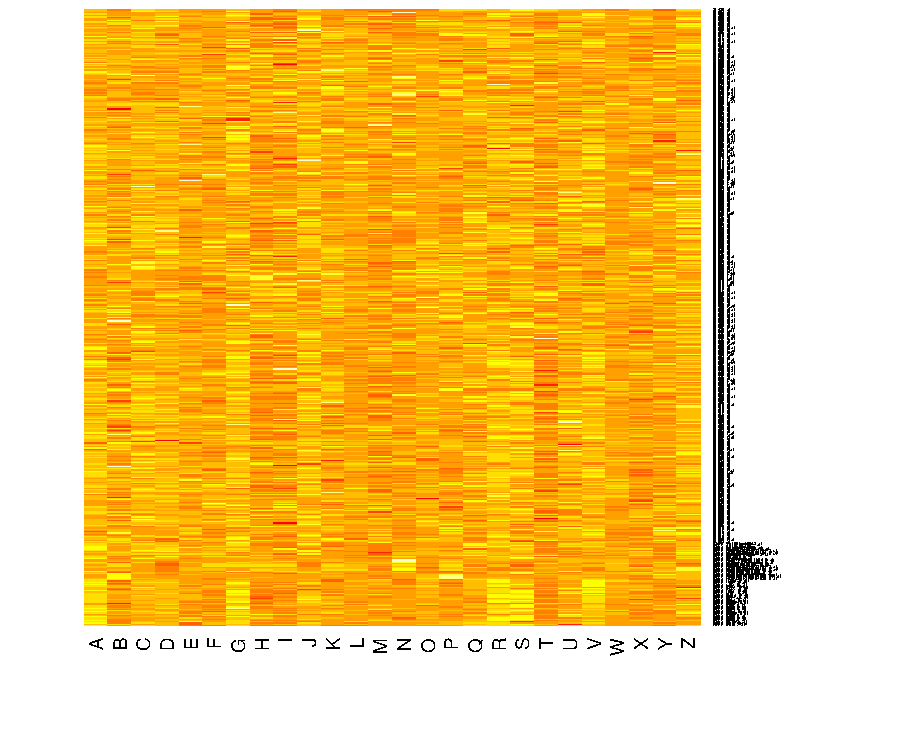
\includegraphics{plots/fig-006}
\end{frame}

\begin{frame}[allowframebreaks, fragile]
  \frametitle{Like \pl{image}?}
  \begin{itemize}
  \item What does \BIOCfunction{heatmap} do to our data before plotting it? 
\begin{Schunk}
\begin{Sinput}
> `?`(heatmap)
\end{Sinput}
\end{Schunk}
  \item Play around with the previous plot:
  \begin{enumerate}
  \item Delete the \pl{Colv} argument
  \item Delete the \pl{Rowv} argument while keeping \pl{Colv}
  \item Delete both and only keep \pl{cexRow}
  \end{enumerate} 
  \item Are all the heatmaps equal? If not, what changes?
  \end{itemize}
\end{frame}

\begin{frame}[allowframebreaks]
  \frametitle{Quick heatmap explanation}
  \begin{itemize}
  \item We won't get into the details, but heatmap with the default parameters re-orders the rows and the columns and creates groups (clusters) determined by euclidean distance.
  \item At some point in the course you'll be able to do heatmaps just like the following one.
  \end{itemize}
\end{frame}

\begin{frame}[fragile]  
  \frametitle{A full heatmap}
  \begin{figure}
  \centering
  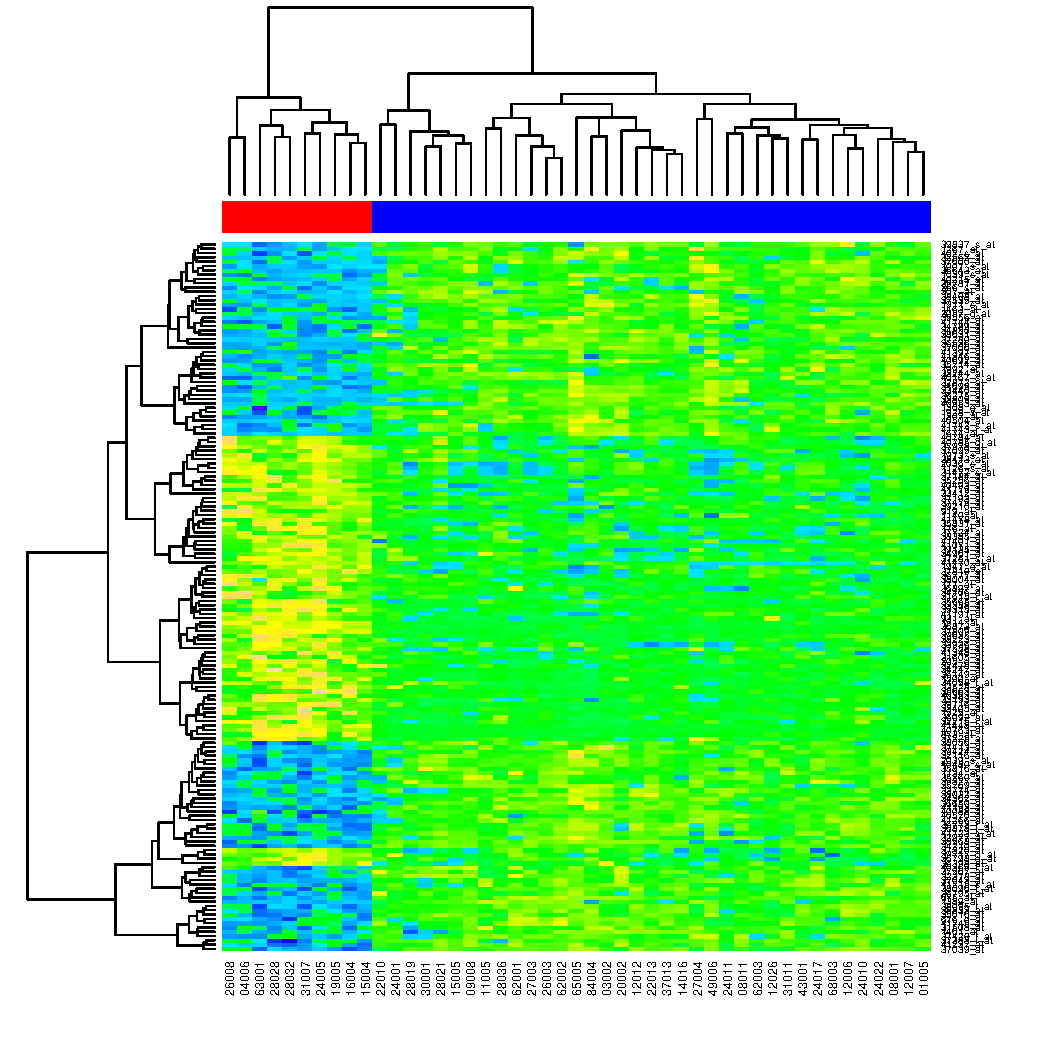
\includegraphics[width=0.8\textwidth, height=0.9\textheight]{heatmap}
  \end{figure}
\end{frame}

%%%%%%%%%%%%%%%%%%%%%%%%%%%%%%%%%%%%%%%%%%%%%%%%%%%%%%%%%%%%%%%%%%%%%%%%%%%
\section{Reproducible Research}

\begin{frame}[allowframebreaks]
  \frametitle{What is it?}
  \begin{itemize}
  \item The goal is simple: to enable others to reproduce your results.
  \item But, isn't research supposed to be reproducible in order to be published? What about supp. material?
  \item \emph{Discussion:} Is it to use the exact same scripts/programs with the same parameters? Or is it to follow the same workflow even if you re-write the scripts?
  \end{itemize}
\end{frame}

\begin{frame}[allowframebreaks]
  \frametitle{Discussion cont.}
  \begin{itemize}
  \item If you don't get the same results using the same scripts/programs and parameters, then something is \alert{seriously} wrong! Or you are not using the same input files; could be a version issue.
  \item Whom do you \emph{\BIOCfunction{trust}}? The one who did the original work or the one who re-wrote the scripts/programs to match the same workflow?
  \end{itemize}
\end{frame}

\begin{frame}[allowframebreaks]
  \frametitle{Discussion cont.}
  \begin{itemize}
  \item Everyone and anyone makes simple mistakes: typos, starting from 0 instead of 1, positive as negative and vice versa, etc.
  \item You can \emph{inherit} problems! Simple enough, you are using data from a previous work and the data has some errors.
  \end{itemize}
\end{frame}

\begin{frame}[allowframebreaks]
  \frametitle{\emph{Forensic} bioinformatics}
  \begin{itemize}
  \item No, it's not to figure out who was the murderer in a crime scene.
  \item Its deciphering someone's code when its messy and the code doesn't match the written description of the algorithm/workflow.
  \item If you aren't careful, you might end up doing forensic bioinformatics with your own code!!! I do recommend using a version control system such as \BIOCfunction{subversion} for your scripts.\footnote{RapidSVN is a simple GUI if you want to avoid the command line}
  \end{itemize}
\end{frame}

\begin{frame}[allowframebreaks]
  \frametitle{Some extreme cases}
  \begin{itemize}
  \item Keith Baggerly gave an excellent talk on the subject at BioC2009. Find it through the workshops site.
  \item 1 to 0 mistakes, adding 1 to names, inverting positive and negative responses, wrong association between names and data, \alert{manual} input of the biological relevant genes, and overall a big mess!!
  \item Magazines didn't seem to care much as no \emph{fe de erratas} was published. Keeping themselves "clean" on public eyes.
  \item Funding agencies see these events \emph{frequently} and they do care more. However, on Baggerly's case study, the scientists are proceeding to experiment with humans\ldots
  \end{itemize}
\end{frame}


\begin{frame}[allowframebreaks]
  \frametitle{So\ldots}
  \begin{itemize}
  \item So, in \pl{R}, how do you do reproducible research?
  \item An excellent practice would be to develop a experimental data package and submit it every time you publish your work. 
  \item You might just use the package to share the data with your lab members or collegues. 
  \item Vignettes! (Sweave is behind)
  \end{itemize}
\end{frame}

\subsection{Sweave}

\begin{frame}[allowframebreaks]
  \frametitle{TEH solution}
  \begin{itemize}
  \item Developed by \myurlshort{www.statistik.lmu.de/~leisch/}{Friedrich Leisch}\footnote{He is a BioC core dev.}, \BIOCfunction{Sweave} is an \pl{R} function that evaluates \pl{R} code chunks and parses the output into \LaTeX format.
  \item \LaTeX files look like a mix between a script and a plain text file. You can turn \LaTeX files into PDF files, just like this presentation and the vignette files!
  \item The workflow is basically:
  \begin{enumerate}
  \item Create a \pl{.Rnw} file in \LaTeX format with some \pl{R} code specified as such.
  \item Transform your \pl{.Rnw} file into a \pl{.tex} file using \pl{Sweave}.
  \item Create the final \pl{.pdf} file from the \pl{.tex} file.
  \end{enumerate}
  \end{itemize}
\end{frame}

\begin{frame}[allowframebreaks]
  \frametitle{Commands in Unix}
  \begin{itemize}
  \item \pl{R CMD Sweave file.Rnw}
  \item \pl{R CMD Stangle file.Rnw}\footnote{Stangle extracts the R code pieces and creates a \pl{.R} file with the \pl{R} code}
  \item \pl{pdflatex file.tex}
  \item \pl{pdftalex file.tex}\footnote{Yes, two times. You need to do so for structures such as the outline.}
  \item If you wish, you can then remove some of the files using \pl{rm}. To avoid typing, it's very useful to create a general shell script :)
  \end{itemize}
\end{frame}

\begin{frame}[allowframebreaks]
  \frametitle{In Windows}
  \begin{itemize}
  \item You will need to install \myurlshort{miktex.org/}{Miktex}. The first time you use pdflatex, Miktex will download some \LaTeX packages.
  \item The commands themselves change such as \pl{R.exe -e "Sweave('file.Rnw')"} and \pl{pdflatex.exe file.tex}\footnote{You might need to modify your PATH environment variable to include the R and R/lib folders}
  \item \url{www.johndcook.com/troubleshooting_sweave.html} is very useful for Windows users.
  \end{itemize}
\end{frame}

\begin{frame}[allowframebreaks]
  \frametitle{User guides}
  \begin{itemize}
  \item We won't go \BIOCfunction{deep} in class time into \LaTeX nor Beamer\footnote{It's used to make presentations such as this one}, but I have cited some very good pdf manuals on the supporting material of this course. 
  \item The Not so Short guide to \LaTeX is very complete :) Check it out for tips on typesetting text and mathematical formulae as well as for a \LaTeX introduction.
  \item There is a second PDF specialized on symbols\ldots and there are LOTS.
  \item Finally, the Beamer User Guide has all you need to know about Beamer and has a funny tutorial.
  \end{itemize}
\end{frame}

\begin{frame}[allowframebreaks]
  \frametitle{Exploring a Rnw file}
  \begin{itemize}
  \item Now, I got started by comparing the \pl{Rnw} files with the pdf files from James Bullard course. And if I had a question, I would check the pdf guides.
  \item To understand more about Sweave, lets check a \alert{Rnw file}. Open \url{www.lcg.unam.mx/~lcollado/B/quizes/01_answer/}
  \item You'll notice the \pl{Sweave.sty} file, which you normally need on every sweave working directory.
  \end{itemize}
\end{frame}

\begin{frame}[allowframebreaks]
  \frametitle{Top of the Rnw file}
  \begin{itemize}
  \item Open the Rnw file. The \% symbol is used to comment lines in \LaTeX, so which is the first un-commented line?
  \item Next we load some \LaTeX packages, define some commands, set the page style and bibliography style.
  \item What do you think the \pl{SweaveOpts} line does?
  \end{itemize}
\end{frame}

\begin{frame}[allowframebreaks, fragile]
  \frametitle{\pl{R} code chunks}
  \begin{itemize}
  \item To avoid spamming our folder, we save the images on the \BIOCfunction{plots} folders with the name starting by \pl{fig}.
  \item I do not recommend having multiple Rnw files on the same working directory. I sometimes use 2 but I need to be careful and specify different figure surnames.
  \item Then we have our first \pl{R} command:
\begin{Schunk}
\begin{Sinput}
> options(width = 40)
\end{Sinput}
\end{Schunk}
  \item As you can see, an \pl{R} code chunk starts with a line \pl{$<$$<$eval=TRUE, echo=TRUE$>$$>$$=$}. Then you can put any \pl{R} code, and you end the chunk with the symbol @.
  \end{itemize}
\end{frame}

\begin{frame}[allowframebreaks]
  \frametitle{The rest of the doc}
  \begin{itemize}
  \item Next, On this Rnw file you'll find information on the title, the author, the start of the document, how to make the title, some line escapes, notes and the abstract.
  \item A file can be divided into \BIOCfunction{sections} and subsections.
  \item Check out the special syntax to include \pl{R} figures.
  \item Remember that for every \pl{begin} there must be an \pl{end} or it'll crash.
  \item The rest should be self explanatory including when the document ends.
  \end{itemize}
\end{frame}

\begin{frame}[allowframebreaks, fragile]
  \frametitle{Workspace}
  \begin{itemize}
  \item Be \alert{careful} with your workspace when using Sweave.
  \item If you have saved a workspace on your current working directory, when you use Sweave it'll be loaded automatically.
  \item You can always add this code line to avoid inheriting workspace issues:
\begin{Schunk}
\begin{Sinput}
> rm(list = ls())
\end{Sinput}
\end{Schunk}
  \end{itemize}
\end{frame}

\subsection{\pl{weaver} package}

\begin{frame}[allowframebreaks]
  \frametitle{A Sweave complement}
  \begin{itemize}
  \item On Bioconductor you can find the \BIOCfunction{weaver} package.
  \item It was designed to help you when your document is large and/or you have time consuming computations that you don't want to repeat every time you change a detail on your Rnw file.
  \item Quite helpful for writing a thesis or some other long project.
  \item Install it with \pl{biocLite} and check out the vignettes; specially the \emph{howto}. 
  \end{itemize}
\end{frame}

\begin{frame}[allowframebreaks, fragile]
  \frametitle{Weaver \pl{R} chunks}
  \begin{itemize}
  \item To use \BIOCfunction{weaver}, you'll need to load it at the beginning.
\begin{Schunk}
\begin{Sinput}
> library(weaver)
\end{Sinput}
\end{Schunk}
  \item Then, your \pl{R} code chunks will start with:
  \item \pl{$<$$<$eval=TRUE, echo=TRUE, cache=TRUE$>$$>$$=$}
  \end{itemize}
\end{frame}


%%%%%%%%%%%%%%%%%%%%%%%%%%%%%%%%%%%%%%%%%%%%%%%%%%%%%%%%%%%%%%%%%%%%%%%%%%%
\section{Exercises/Homework}

\begin{frame}[allowframebreaks]
  \frametitle{Part 1: template}
  Create your own template Sweave document.
  \begin{itemize}
  \item Title: course name, homework number
  \item Author: name, email, include a link to your personal academic webpage if you have one.\footnote{You will probably make one this semester on the PHP course.}
  \item Abstract: short description on the homework and any notes you might want to add
  \item A sample homework solution: meaning a short description and some code. For example, how to sum $2 + 3$.
  \end{itemize}
\end{frame}

\begin{frame}[allowframebreaks, fragile]
  \frametitle{Part II: \emph{ALL} dataset}
  \begin{itemize}
  \item You'll have to explore the ALL dataset\footnote{John Quackenbush mentioned it on Monday as the most studied dataset.} and create your first homework as a vignette document.
  \item Install the \BIOCfunction{ALL} package and explore the \pl{ALL} object.
\begin{Schunk}
\begin{Sinput}
> library(ALL)
> data(ALL)
\end{Sinput}
\end{Schunk}
  \item Select the samples from the B-cell tumors.
  \item Select those of molecular type \pl{BCR/ABL} or \pl{NEG}.
  \item Combine the previous two subsets and keep the \emph{intersect}ion
  \item Eliminate unused factor levels on your resulting subset.
  \item Use the \BIOCfunction{nsFilter} function from the \pl{genefilter} package to keep those with \emph{entrez} ID, \emph{GOBP}, remove duplicate \emph{entrez} and the following arguments:
\begin{Schunk}
\begin{Sinput}
> nsFilter(var.fun = IQR, var.cutoff = 0.5, 
+     feature.exclude = "^AFFX")
\end{Sinput}
\end{Schunk}
  \item Meaning that we'll use the interquantile range with a variance cutoff of 0.5 to eliminate those with small variation and by excluding \pl{AFFX} we'll take out the controls AFFY probes.
  \item How many:
  \begin{enumerate}
  \item duplicates were removed?
  \item control features were excluded?
  \item had low variance (small variation)?
  \item had no GO?
  \item had no entrez ID?
  \end{enumerate}
  \end{itemize}
\end{frame}

\begin{frame}[allowframebreaks, fragile]
  \frametitle{Session Info}
  \scriptsize
\begin{Schunk}
\begin{Sinput}
> sessionInfo()
\end{Sinput}
\begin{Soutput}
R version 2.10.0 Under development (unstable) (2009-07-25 r48998) 
i686-pc-linux-gnu 

locale:
 [1] LC_CTYPE=en_US.UTF-8      
 [2] LC_NUMERIC=C              
 [3] LC_TIME=en_US.UTF-8       
 [4] LC_COLLATE=en_US.UTF-8    
 [5] LC_MONETARY=C             
 [6] LC_MESSAGES=en_US.UTF-8   
 [7] LC_PAPER=en_US.UTF-8      
 [8] LC_NAME=C                 
 [9] LC_ADDRESS=C              
[10] LC_TELEPHONE=C            
[11] LC_MEASUREMENT=en_US.UTF-8
[12] LC_IDENTIFICATION=C       

attached base packages:
[1] stats     graphics  grDevices
[4] utils     datasets  methods  
[7] base     

other attached packages:
[1] Biobase_2.5.5

loaded via a namespace (and not attached):
[1] tools_2.10.0
\end{Soutput}
\end{Schunk}
\end{frame}

\end{document}
